\documentclass[12pt,twocolumn]{article} 

% required packages for Oxy Comps style
\usepackage{oxycomps} % the main oxycomps style file
\usepackage{times} % use Times as the default font
\usepackage[style=numeric,sorting=nyt]{biblatex} % format the bibliography nicely

\usepackage{amsfonts} % provides many math symbols/fonts
\usepackage{listings} % provides the lstlisting environment
\usepackage{amssymb} % provides many math symbols/fonts
\usepackage{graphicx} % allows insertion of grpahics
\usepackage{hyperref} % creates links within the page and to URLs
\usepackage{url} % formats URLs properly
\usepackage{verbatim} % provides the comment environment
\usepackage{xpatch} % used to patch \textcite

\bibliography{references}
\DeclareNameAlias{default}{last-first}

\xpatchbibmacro{textcite}
  {\printnames{labelname}}
  {\printnames{labelname} (\printfield{year})}
  {}
  {}

\pdfinfo{
    /Title (Experiencing Mexican Culture through cuisine in VR)
    /Author (Justin Li)
}

\title{Experiencing Mexican Culture through cuisine in VR}

\author{Stephanie Enriquez Isais}
\affiliation{Occidental College}
\email{senriquezisa@oxy.edu}

\begin{document}

\maketitle

\begin{abstract}
    This document serves as an introduction to {\LaTeX} and also describes the requirements of the senior project final paper for Occidental College's Computer Science majors.
    We start by justifying the use of {\LaTeX} over Word, Google Docs, and other What-You-See-Is-What-You-Get (WYSISYG) editors.
    A brief tutorial to {\LaTeX} follows, reviewing the most common commands used in paper writing.
    We then turn our attention to the Oxy CS Comps Paper, first contextualizing it within the major curriculum, before exploring each major section of the paper in detail.
    We conclude with some miscellaneous tips for successfully completing comps.
\end{abstract}

\section{Problem Context}
There are 69 official languages in Mexico and each of it’s 32 states has its own distinct traditions, style and cuisine. From an outsider’s perspective, Mexican culture is often just associated with sombreros, tacos, burritos, and tequila, and while these do make up a part of Mexican culture, they are nowhere near representative of all Mexico has to offer. Mexican cuisine is extremely diverse and has a lot of historical significance. There are drinks, like tepache (fermented pineapple juice), that have pre colonial roots and are still widely enjoyed by people in Mexico. However, unless you live in Mexico or have some Mexican heritage you probably won’t ever encounter these parts of Mexican culture. In addition to that, the way Mexican food was prepared in the past is not prevalent even in the average Mexican household. Tools like the metate (mealing stone) where used by Mexican people in the past to breakdown their corn or other ingrediatn into a fine powder. The word metate comes from the Nauhuatl word metlatl which means grinding stone. The indigounse Mexican people of the past use metates to grind the Maize down and be able to make tortillas. These tools and techniques have historical value to the Mexican culture and should not be forgotten. Evne when talking to my Mexican American friends, alot of them don’t know what a metate is, but their grandparents or even parents probably do know what it is and how it was used. Although most mexican household have replace the metate with a food processor or a molcajete (pestel and mortar) there are a couple of people who still use them. My dad tells me about the metate my grandmother was given when she got married and the pride she took in how much use she got out of it and the unique taste it gave her food. This is the historical contect that I want to teach people about. Although VR does not provide a way to showcase the unique taste and labor that goes into using these Mexican tools, I still think it’s a great way of getting people interested in the historical importance of them. They shaped Mexican culture and offer Mexicans a way of staying connected to our indigounes roots. 

\section{Technical Background}

\section{Prior Work}
When doing research into the prior work done in to address this problem, I found a couple of VR apps that are related to my VR project idea. The first one is called Lost Recipes, this VR game taeches user show to many an array of traditional dishes from ancient cultures like the Mayan, Greek and Chinese. The game guides the players through tasks like measure and mixing ingraidenats in an effort to recreate a traditional recipe. While this game does a good job of encouraging the users to complete the tasks and even try the recipes out on their own (thsi is based off some reviews left on the game), it doesn’t give much historical information about the significance of the food or tools they are using. Since this is the game that is most similar to my idea, it has helps me identify the areas that I would like to improve on. At the same time, playing the game has taught me about the manner in which affordances can be used to have the user complete the game in the intended manner and gain the most out of it. Another similar cooking game is Cooking Simulator. As the name suggests this game is alot more focused on creating a realistic experience of what it is like to cook in VR. The user has to measure each ingredient, can cut the produce and can even cook or bake in the game. This game is a probably one of the most realistic cooking simulators and gives good examples of hwo to program the tools in the kitchen so the user can use them with controllers. When looking at references for how to build my cooking mechanics I think this game will be a great example to look back upon. In addition to the cooking aspect of my project, I want to reall take advantage of the immerisnvess of VR and create a VR experience that can tells a story in a more engaging way. The first example is the VR game “Vader Immortal”. The game revolves around the player trying to stop Darth Varder from completely destroying the planet Mustafar. When presenting the player with the history of the planet and why they should fight for it, they do it through the use of 3D animations. The majority of the game is the user traveling, flighting and exploring the world but when presenting what is at stake, the creators decided to use storytelling through animation and after playing the game, it is clear why they made this choice. Seeing the storying quite literally unravel around you makes it more engaging and immersive. It inspires me to create a similar sentiment when describing the history of Mexican cuisine. The Vader immortal approach to story telling is similar to the cutscenes that are often used in videogames but another technique for storytelling that would be interesting is the one the VR game “What Remains of Edith Finch”. This game details the stories about what happened to the Finch family and one scene does this very interesting of incporting the mundane chore of cutting fish heads in a assembly line with their daydreams slowly taking up more and more of the screenspace. I think incorporating something similar to this in which the user is using one of the labor intensive cooking tools and then they see a scene of the history of the ingredients theu are using would be an interersing way of engaging he user witht he content I am trying to teach htem about. 
 


\section{Using \LaTeX}

LaTeX (pronounced \textit{lah-teck} or \textit{lay-teck}), often stylized as {\LaTeX} and written as latex, is a document markup language and typesetting system.
Building on the {\TeX} language created by Donald Knuth in 1978, LaTeX provides additional commands for common document needs such as sections, figures, and bibliograhpies.
LaTeX is widely used in academia, especially in mathematical fields, due to how easy it is to write mathematical equations and its automatic management of references.
Since it is a markup language, LaTeX source files are written in plain text, which also makes it compatible with version control systems like git.

The most primitive syntax of LaTeX is the \textit{macro} or \textit{command}, which is always written with a backslash followed by the name of the command.
The {\LaTeX} glyph, for example, can be created with the command \texttt{\textbackslash LaTeX}.
Some commands take parameters, which are denoted in braces (e.g., \texttt{\textbackslash usepackage\{biblatex\}} will import the \texttt{biblatex} package), with some commands additionally accepting options in square brackets (e.g., \texttt{\textbackslash usepackage[style=numeric]\{biblatex\}}).
The \texttt{\textbackslash begin} and \texttt{\textbackslash end} commands are special, as they indicate the start of an \textit{environment}.
The content of LaTeX documents, for example, are surrounded by \texttt{\textbackslash begin\{document\}} and \texttt{\textbackslash end\{document\}}, indicating the text that should appear in the document.

\begin{figure}
    \centering
    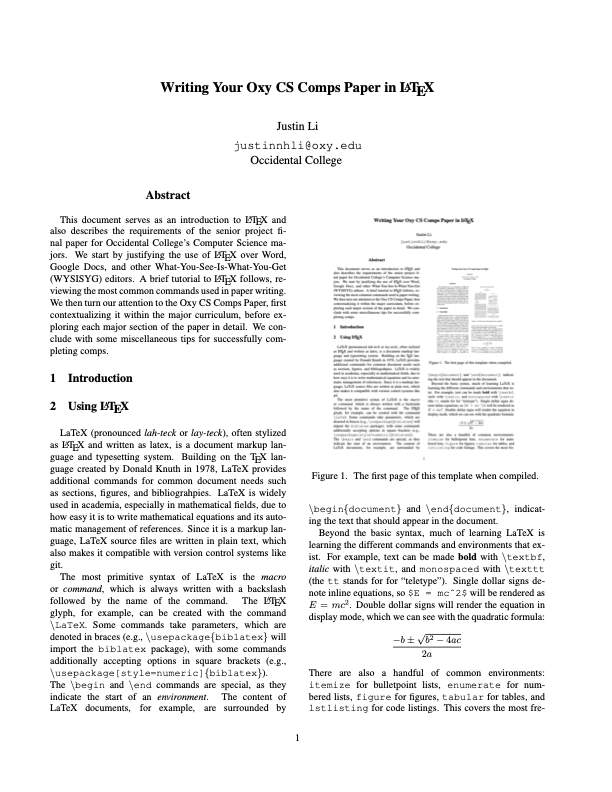
\includegraphics[width=.95\linewidth]{first-page.png}
    \caption{
        The first page of this template when compiled.
    }
    \label{structures}
\end{figure}

Beyond the basic syntax, much of learning LaTeX is learning the different commands and environments that exist.
For example, text can be made \textbf{bold} with \texttt{\textbackslash textbf}, \textit{italic} with \texttt{\textbackslash textit}, and \texttt{monospaced} with \texttt{\textbackslash texttt} (the \texttt{tt} stands for for ``teletype'').
Single dollar signs denote inline equations, so \texttt{\$E = mc\textasciicircum 2\$} will be rendered as $E = mc^2$.
Double dollar signs will render the equation in display mode, which we can see with the quadratic formula:
$$\frac{{-b \pm \sqrt {b^2 - 4ac} }}{{2a}}$$
There are also a handful of common environments: \texttt{itemize} for bulletpoint lists, \texttt{enumerate} for numbered lists, \texttt{figure} for figures, \texttt{tabular} for tables, and \texttt{lstlisting} for code listings.
This covers the most frequently used commands, but as you might have already inferred, LaTeX is a vast and deep system, and can easily be overwhelming.
We recommended following the \citetitle{Overleaf2021LearnLaTeXIn} tutorial \cite{Overleaf2021LearnLaTeXIn}, and examining and playing with the source of this document, to gain working proficiency with LaTeX.

One final note on writing in LaTeX.
Since LaTeX is only a markup language, the source files must be compiled into a viewable form, most commonly into a PDF file.
The source of this document is made up of several files, each with its own purpose:
\begin{itemize}
    \item \texttt{template.tex} - The main LaTeX file containing the contents of the document.
    \item \texttt{oxycomps.sty} - A style file with settings for what the document should look like.
    \item \texttt{references.bib} - A list of bibliography items.
    \item Other files containing images, build instructions, etc.
\end{itemize}
Manual compilation of these files is somewhat esoteric, as it requires multiple uses of the \texttt{pdflatex} and \texttt{biblatex} commands.
Instead, it is much easier to use tools such as \texttt{latexmk} (in the terminal) or Overleaf (online) for compilation.
We have also provided a \texttt{Makefile} which will automatically update the document as necessary; the use of makefiles is beyond the scope of this document, but see \textcite{Lambert2021MakefileTutorial}.

\begin{comment}

\begin{figure}[]
    \begin{center}
        \includegraphics[width=\linewidth]{figure.pdf}
    \end{center}
    \caption{
        Figure caption.
        To get a figure to span two columns, use the {\tt figure*} environment rather than {\tt figure}.
    }
    \label{figure1}
\end{figure}

\begin{quote}
    Lorem ipsum dolor sit amet, consectetur adipiscing elit.
    Mauris pellentesque est nec nunc fringilla, a finibus nisl tempor.
    Sed semper est massa, eget pulvinar neque posuere id.
    Ut mauris tellus. 
\end{quote}

\begin{lstlisting}[language=Python]
def hello():
    print('hello, world!')
\end{lstlisting}

\end{comment}

\begin{comment}
No definition citations, unless the term itself is in dispute
Separate problem background from technical background
    Unclear if games and apps require much technical background
    The general structure of the framework might be better suited for the Architecture Overview section
        Eg. Flask uses decorators to associate functions with URLs
        Eg. Unity has scripts associated with objects and specific triggers, such as walking into an area, pressing a button, etc.
    Maybe a better name is "algorithmic background"?
        Should explore what does and doesn't count
            All ML counts
            App and game frameworks do not
        Framework vs. library?
            I like the idea of [inversion of control](https://martinfowler.com/bliki/InversionOfControl.html), but that may be too abstract for students to understand
        Heuristic: is understanding that system necessary to understand the results?
            Ie. How Flask or Unity works doesn't influence whether the app/game is useful/fun/engaging
            But how (say) linear regression works is highly relevant for why the results match/don't match the actual values
\end{comment}

\printbibliography 

\end{document}
